% Operations Nerd — Updated HLD (v2)
% Senior researcher's response to the junior's v1 proposal
% Trimmed, realistic, designed for printing/sharing as PDF.

\documentclass[11pt,a4paper]{article}

% Geometry & layout
\usepackage[a4paper,margin=2.2cm,headheight=16pt,top=2.4cm,bottom=2.2cm]{geometry}
\usepackage{microtype}
\usepackage{parskip}
\setlength{\parskip}{6pt}
\setlength{\parindent}{0pt}
\usepackage{enumitem}
\setlist{topsep=2pt,itemsep=1pt,parsep=0pt}

% Color palette — slate-blue accent + warm neutrals
\usepackage{xcolor}
\definecolor{accent}{HTML}{2C5F8D}
\definecolor{accentlight}{HTML}{E6EEF6}
\definecolor{warmrule}{HTML}{C9B8A0}
\definecolor{codebg}{HTML}{F6F2EC}
\definecolor{ink}{HTML}{1F2933}
\definecolor{inkmuted}{HTML}{5A6470}

\usepackage{hyperref}
\hypersetup{colorlinks=true,linkcolor=accent,urlcolor=accent,citecolor=accent,
  pdftitle={Operations Nerd — Updated HLD (v2)},
  pdfauthor={Senior Researcher},
  pdfsubject={Internal HLD review}}
\color{ink}

% Typography
\usepackage[T1]{fontenc}
\usepackage[utf8]{inputenc}
\usepackage{lmodern}
\usepackage{textcomp}

% Tables
\usepackage{booktabs}
\usepackage{tabularx}
\usepackage{array}
\renewcommand{\arraystretch}{1.15}
\usepackage{colortbl}

% Code (lightweight, no listings dep needed)
\usepackage{tcolorbox}
\tcbuselibrary{skins,breakable}
\newtcolorbox{codebox}{
  enhanced, breakable,
  colback=codebg, colframe=warmrule,
  boxrule=0.4pt, arc=2pt, left=8pt, right=8pt, top=5pt, bottom=5pt,
  fontupper=\ttfamily\footnotesize, fontlower=\ttfamily\footnotesize,
  before skip=6pt, after skip=6pt,
}

% Headers & titles (tighter spacing)
\usepackage{titlesec}
\titleformat{\section}
  {\large\bfseries\color{accent}}
  {\thesection}{0.6em}{}
  [\vspace{-3pt}\color{warmrule}\hrule height 0.5pt]
\titleformat{\subsection}
  {\normalsize\bfseries\color{accent}}
  {\thesubsection}{0.5em}{}
\titlespacing*{\section}{0pt}{14pt}{6pt}
\titlespacing*{\subsection}{0pt}{10pt}{3pt}
% Unnumbered section style — no rule, no number, smaller
\newcommand{\unnumsec}[1]{%
  \par\addvspace{10pt}%
  {\large\bfseries\color{accent} #1\par}%
  \addvspace{2pt}%
  \nopagebreak
}

% Page header
\usepackage{fancyhdr}
\pagestyle{fancy}
\fancyhf{}
\fancyhead[L]{\small\itshape\color{inkmuted}Operations Nerd — HLD v2}
\fancyhead[R]{\small\color{inkmuted}\nouppercase{\leftmark}}
\fancyfoot[C]{\small\color{inkmuted}\thepage}
\renewcommand{\headrule}{\color{warmrule}\hrule height 0.4pt}

% TikZ for the 3-planes diagram
\usepackage{tikz}
\usetikzlibrary{positioning,arrows.meta,calc,fit}
\tikzset{
  plane/.style={rectangle, rounded corners=2pt, draw=accent, fill=accentlight,
                align=left, inner sep=7pt, text width=4.3cm,
                font=\footnotesize},
  corenode/.style={rectangle, rounded corners=2pt, draw=accent!70, fill=white,
                   align=center, inner sep=5pt, text width=11.5cm,
                   font=\footnotesize\itshape},
}

\title{}
\author{}
\date{}

\begin{document}

% --- Title block ---
\begin{tcolorbox}[
  enhanced, colback=accent, colframe=accent, arc=2pt, boxrule=0pt,
  left=16pt, right=16pt, top=10pt, bottom=10pt,
  borderline west={3pt}{0pt}{white},
  fontupper=\color{white}
]
  {\LARGE\bfseries Operations Nerd — Updated HLD (v2)}\par
  \vspace{1pt}
  {\small A senior's read of the v1 proposal. Trimmed, opinionated, ready to share.}
\end{tcolorbox}

\vspace{2pt}
\begin{center}
  \small\color{inkmuted}
  Senior researcher · 2026-07-25 · for the junior author (primary) and Prof.\ Sasha
\end{center}

\vspace{2pt}
\markboth{}{Summary}
\unnumsec{v1 in one breath}
Right thesis (config-first, shared ontology, vertical adapter). Thin
substrate: four-primitive ontology, no data model, no multi-tenant story,
no reliability layer for side effects, no HITL design, no eval plan, and
the nine-stage pipeline conflates one-time setup with per-event processing.

\unnumsec{v2 in one breath}
Same thesis, real engineering. Adds a two-layer ontology, Postgres RLS
multi-tenancy, transactional outbox + saga, durable execution on
Temporal+LangGraph, an explicit HITL gate with three-signal confidence, a
git-shaped snapshot model, and a continuous discovery loop. The nine
stages split into a \emph{one-time onboarding pipeline} and a
\emph{per-event runtime pipeline}.

% --- Three planes ---
\section{Three planes, three cadences}

The runtime is not one pipeline, it's three. v1's stage 7 was actually
onboarding, not a per-event stage; v2 makes that explicit.

\begin{center}
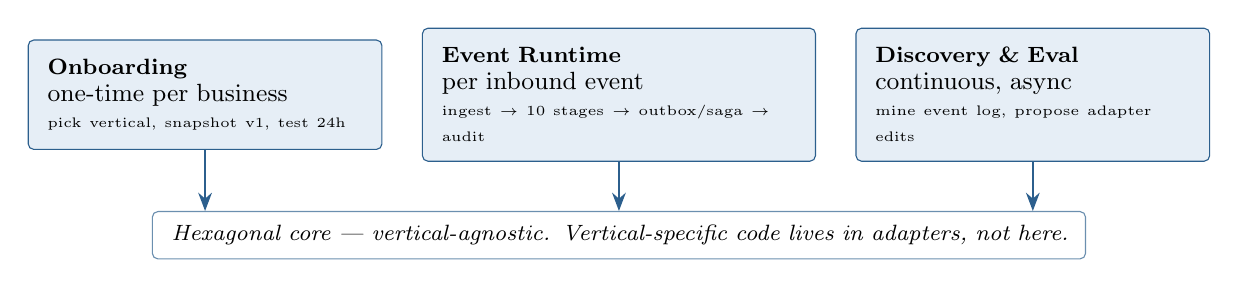
\begin{tikzpicture}[node distance=0.55cm]
  \node[plane, text width=4.0cm] (p1) {\textbf{Onboarding}\\{\small one-time per business}\\{\tiny pick vertical, snapshot v1, test 24h}};
  \node[plane, right=0.5cm of p1, text width=4.5cm] (p2)
        {\textbf{Event Runtime}\\{\small per inbound event}\\{\tiny ingest $\to$ 10 stages $\to$ outbox/saga $\to$ audit}};
  \node[plane, right=0.5cm of p2, text width=4.0cm] (p3)
        {\textbf{Discovery \& Eval}\\{\small continuous, async}\\{\tiny mine event log, propose adapter edits}};

  \node[corenode, below=0.7cm of $(p1.south)!0.5!(p3.south)$] (core)
        {Hexagonal core — vertical-agnostic. Vertical-specific code lives in adapters, not here.};
  \draw[->, >=Stealth, color=accent, thick] (p1.south) -- (p1.south |- core.north);
  \draw[->, >=Stealth, color=accent, thick] (p2.south) -- (core.north);
  \draw[->, >=Stealth, color=accent, thick] (p3.south) -- (p3.south |- core.north);
\end{tikzpicture}
\end{center}

The core follows \emph{Ports \& Adapters} (Cockburn): vertical-specific
code is an adapter. Anything that differs per business lives in the
saved-state snapshot; anything that doesn't stays in the core.

% --- Per-event pipeline ---
\sectionmark{Per-event pipeline (10 stages)}
\section{Per-event runtime pipeline (10 stages)}

v1's stages 7--9 were actually onboarding, not runtime. v2 splits them
out cleanly. The runtime is ten stages end-to-end, every stage writes an
append-only \texttt{Event} row, and the last two stages run in parallel
after the action lands.

\begin{center}
\renewcommand{\arraystretch}{1.15}
\begin{tabularx}{\linewidth}{@{}p{0.55cm}p{3.3cm}X@{}}
\toprule
\rowcolor{accentlight}\textbf{\#} & \textbf{Stage} & \textbf{What it does (and the failure guard)}\\
\midrule
1 & Ingest                 & Webhook / polling / CSV arrives. Idempotency row by \texttt{(tenant, source, source\_event\_id)}. Dedupe. \\
2 & Validity Gate          & Confirm legitimate event (not spam, not malformed). LLM-as-judge + rule prefilter. \\
3 & Ontology Conversion    & Map to upper-core entities (Party / Engagement / Agreement / Transaction / Obligation / Event). JSON-Schema validated. \\
4 & Context Extraction     & Read prior records, related entities, calendar, payment status. Read-only Temporal activity. \\
5 & Function Classification& Route to relationship / sales / outreach / accounting. Constrained LLM + rule fallback. \\
6 & Compliance \& Safety   & Pluggable: OPA/Rego rules, LLM-as-judge, HITL escalation. All decisions logged to audit. \\
7 & Action Drafting        & Produce typed action object (\texttt{SendEmail}, \texttt{PostInvoice}, \dots). Pure object, never executed. \\
8 & HITL Gate              & \emph{auto} / \emph{requires\_approval} / \emph{block} per action type. Three-signal confidence threshold. \\
9 & Action Execution       & Outbox row + state change in \emph{one} DB transaction. Idempotency four-tuple. Saga compensations. \\
10a & Audit Log           & Append \texttt{Event} row (XES-extended). Drives discovery + compliance audit + drift monitor. \\
10b & Live Feedback       & SSE stream to the Web Console, per \texttt{event\_id}, stage-by-stage. \\
\bottomrule
\end{tabularx}
\end{center}

% --- Snapshot model ---
\sectionmark{Saved-state snapshot}
\section{Saved-state snapshot (the actual deliverable)}

Per-business adapter state, versioned like git. Immutable blobs in object
storage, pointer + metadata in the DB, hash-checked on every read.
\emph{Anything that differs per business lives here; anything that
doesn't lives in the core.}

\begin{codebox}
\begin{tabbing}
\hspace{0.5cm}\=\hspace{4.5cm}\=\kill
snapshot = \{\\
  \>schema\_version\:      "opsnerd.snapshot.v2",\\
  \>snapshot\_id\:         "snap\_<uuid>",\\
  \>parent\_snapshot\_id\:  "snap\_<uuid>" \,|\, null,           // fork / rollback\\
  \>tenant\_id\:           "<uuid>",\\
  \>provenance\:           "onboarding" \,|\, "discovery\_proposal" \,|\, "manual\_edit" \,|\, "rollback",\\
  \>ontology\:             \{ ... lower-core per vertical ... \},\\
  \>policies\:             \{ ... OPA bundle, action-type approval defaults ... \},\\
  \>action\_templates\:     \{ ... typed action shapes per use case ... \},\\
  \>integrations\:         \{ ... scopes only; tokens live in Vault ... \},\\
  \>hash\:                 sha256(canonical\_json),                 // integrity\\
\}
\end{tabbing}
\end{codebox}

\textbf{Rollback} = load the parent snapshot; in-flight events resume from
their Temporal checkpoint with the parent state loaded. History is
append-only.

% --- The three things that make it production-realistic ---
\sectionmark{The three things that make it production-realistic}
\section{The three things that make it production-realistic}

Without these, the junior's pipeline is a research demo. With them, it's
shippable. The literature is unambiguous on each.

\paragraph{1. Transactional outbox + saga for every side effect.}
CRMArena-Pro (Salesforce, 2025) puts the best LLM agents at 58\%
single-turn / 35\% multi-turn on real CRM tasks. Production-agent
studies (Fiddler, gravity.fast, 2026) put real-world failure rates at
70--95\%, with 88\% of demo-passing agents failing in production. The
fix isn't a better prompt, it's a separate dispatch layer that
guarantees the state change and the external action are atomic. We
write the outbox row \emph{in the same transaction} as the state
change; a separate drainer dispatches. Four-tuple idempotency key
\texttt{(agent\_run\_id, step\_id, tool\_name, business\_scope)}; both
forward and compensation actions are idempotent under the same key.

\paragraph{2. HITL as a first-class subsystem, not a footnote.}
v1 mentioned approval in §4 prose. v2 makes it stages 7--8 with a
three-signal confidence threshold (LLM + rule coverage + historical
accuracy on this action type), default policy
\emph{auto/requires\_approval/block} on a reversibility $\times$ risk
matrix, and a \emph{promote-to-policy} path that turns a one-off
decision into a standing rule. Practitioner data (dev.to, 2026) shows
HITL reduces critical error rate from 23\% to 5.1\% on the same agent
workflow. The human override rate is the most reliable leading
indicator of system quality, alert on trend.

\paragraph{3. Durable execution on Temporal + LangGraph.}
Per LangChain's 1.0 release (Oct 2025) and the 2026 production
consensus: \emph{Temporal} for the outer workflow (retries,
compensations, multi-day waits, cross-service), \emph{LangGraph} for
the inner agent reasoning (cyclical control flow, conditional routing,
checkpoint per node to Postgres). The outbox is the bridge between
"the agent decided" and "the external system was called."

% --- Data model in one breath ---
\sectionmark{Data model + ontology}
\section{Data model and ontology in one breath}

Two-layer ontology. Eight upper-core entities in the core (Party, Party
Relationship, Engagement, Agreement, Transaction, Transaction Line,
Obligation, Event), per-vertical lower-core subclasses in the snapshot.
Every table has \texttt{tenant\_id} + Postgres RLS
(\texttt{FORCE ROW LEVEL SECURITY}, \texttt{app.current\_tenant} GUC
set on the connection). Outbox, saga, approvals, audit\_log, and
snapshots live in the same DB. Integration tokens are encrypted, never
in snapshots.

The two-layer pattern is taken straight from O-CREAM-v2 (Cairns et
al., 2010) and CURIE-O (Sales et al., 2021), the academic CRM
ontologies for SMEs. v1's four primitives can't model real CRM
relationships, audit trails, or event sourcing. Eight upper-core
entities can.

% --- Open questions ---
\sectionmark{Open questions for the junior}
\section{Open questions for the junior}

v3 is gated on answers to these. Pick one, defend the choice in two
paragraphs.

\begin{enumerate}[leftmargin=*,itemsep=3pt]
  \item \textbf{First vertical.} My pick is real estate: lower regulatory
        bar than clinic, higher willingness-to-pay than generic sales,
        and the v1 walkthrough already uses it. Clinic is second-best
        if you want to lead with the higher revenue ceiling.
  \item \textbf{Build vs buy the runtime substrate.} My pick is Temporal
        Cloud + LangGraph 1.0 (managed) to remove a class of operational
        burden in v1. Temporal OSS + custom checkpointer is cheaper at
        scale but eats engineering time. Decide before you write a line
        of runtime code.
  \item \textbf{First saved-state authoring path.} My pick is
        discovery-loop-first: mine the business's first 90 days of
        events to propose a starter snapshot, then the owner reviews and
        edits in the Web Console. Pure hand-authored questionnaire is
        the alternative.
  \item \textbf{Approval default for \texttt{send\_external}.}
        My pick: \emph{requires\_approval} by default for 30 days, then
        owner-configurable to \emph{auto} per action type after a clean
        track record. Never default to \emph{auto}.
  \item \textbf{Relationship to CustomNerd.} My pick is to publish v2 as
        a separate artifact with explicit cross-references in the
        dissertation chapter, not as a CustomNerd extension. The
        engineering substrate (durable execution, outbox/saga, RLS,
        snapshot model) is the difference, and conflating them will
        confuse readers.
\end{enumerate}

\vfill
\noindent{\footnotesize\color{inkmuted}\textbf{Sources:} CRMArena-Pro (Salesforce, 2025) · O-CREAM-v2 · CURIE-O · PMAx/pm4aa (2026) · LangGraph 1.0 · Temporal · Replit snapshot engine · Postgres RLS production patterns · Fiddler / gravity.fast / armalo 2026 practitioner studies. Failure-mode catalog, full RLS schema, and eval plan are in the companion \texttt{Operations-Nerd-HLD-v2.md}.}

\end{document}

